\documentclass[a4paper]{article}
\usepackage[T2A]{fontenc}
\usepackage[utf8]{inputenc}
\usepackage[ukrainian]{babel}
\usepackage{tikz}
\usepackage{lastpage} 
\usepackage[left=2.5cm, right=1.5cm, top=1.5cm, bottom=2.7cm]{geometry}
\usepackage{fancyhdr}
\usepackage{amsmath, amssymb, amstext} % Математичні символи
\usepackage{fp}
\usepackage{ragged2e}

\usepackage{listings}

\usepackage{xifthen} % Для умовних перевірок

% \usepackage{fontspec}
% \setmainfont{Times New Roman}

\usepackage{caption}


% \usepackage{graphicx}

\pagestyle{fancy}
\fancyhf{}
\renewcommand{\headrulewidth}{0pt}
\renewcommand{\footrulewidth}{0pt}

% \pagestyle{empty}

\newcommand{\makrosCalc}[1]{
    \FPeval{\the\fpresult}{#1}
}

\newcommand{\makrosmytitle}[2]{
    \thispagestyle{empty}
    \centering
    \textbf{Міністерство освіти і науки України}\\
    \textbf{КИЇВСЬКИЙ ПОЛІТЕХНІЧНИЙ УНІВЕРССИТЕТ}\\[2cm]
    \raggedleft
    Кафедра автоматизації та систем неруйнівного контролю\\
    Група ПМ-11
    \vfill
    \centering
    \textbf{ПРОЕКТУВАННЯ СИСТЕМ АВТОМАТИЗАЦІЇ}\\[1cm]
    \textbf{ЗВІТ З #1}\\[1cm]
    \textbf{\huge #2}
    \vfill
    \begin{flushleft}
        Керівник  \qquad\qquad\quad \hfill\qquad (підпис)\hfill 
        д.т.н., проф. Черепанська І. Ю.\\
        \hfill (дата)\\[2cm]
        Виконавець\hfill (підпис)\hfill Осипчук О. Г.\\
        \hfill (дата)
    \end{flushleft}
    \vfill
    \centering
    2025
}

\newcommand{\makrosFrameBig}[2]{
    \thispagestyle{empty} % Вимикає номер сторінки на першій сторінці
    
    \begin{tikzpicture}[remember picture, overlay]
        \begin{scope}[shift={([xshift = 20 mm, yshift = 10 mm]current page.south west)}]
            \draw[line width=2] (0,0) rectangle (180 mm,277 mm);
        \end{scope}
    \end{tikzpicture}
    
    \begin{tikzpicture}[remember picture, overlay]
        \begin{scope}[shift={([xshift = 20 mm, yshift = 10 mm]current page.south west)}, x=1mm, y=1mm]
            \draw[line width=2] (0,0) rectangle (180,40);
            \draw[line width=2]  (7,40) -- (7, 25);
            \draw[line width=2] (17,40) -- (17, 0);
            \draw[line width=2] (40,40) -- (40, 0);
            \draw[line width=2] (55,40) -- (55, 0);
            \draw[line width=2] (65,40) -- (65, 0);
            \draw[line width=2] (135,25) -- (135,0);
            \draw[line width=2] (140,15) -- (140,20);
            \draw[line width=2] (145,15) -- (145,20);
            \draw[line width=2] (150,25) -- (150,15);
            \draw[line width=2] (165,25) -- (165,15);
        
            \draw (0,35) -- (65, 35);
            \draw[line width=2] (0,30) -- (65, 30);
            \draw[line width=2] (0,25) -- (180, 25);
            \draw (0,20) -- (65, 20);
            \draw (0,15) -- (65, 15);
            \draw (0,10) -- (65, 10);
            \draw (0,5) -- (65, 5);
        
            \draw[line width=2] (135,20) -- (180, 20);
            \draw[line width=2] (135,15) -- (180, 15);
            
            \node at (3.5, 27.5) {Зм.};
            \node at (12, 27.5) {Лист};
            \node at (28.5, 27.5) {№ докум.};
            \node at (47.5, 27.5) {Підпис};
            \node at (60, 27.5) {Дата};
            
            \node at (7, 22.5) {Розроб.};
            \node at (6.5, 17.5) {Перев.};
            \node at (8.5, 7.5) {Н. Контр.};
            \node[align=left] at (5, 2.5) {Затв.};
            
            \node at (142.5, 22.5) {Літ.};
            \node at (157.5, 22.5) {Аркуш};
            \node at (172, 22.5) {Аркушів};
        
            \node[align=left, font=\itshape, anchor=south west, scale=0.9] at (16, 20) {Погорєлов Б.Ю.};
            \node[align=left, font=\itshape, anchor=south west, scale=0.8] at (16, 15) {Черепанська І.Ю.};
            \node[align=left, font=\itshape, anchor=south west, scale=0.8] at (16, 0) {Черепанська І.Ю.};
        
            \node[anchor=center, font=\itshape, scale=1.5] at (122, 32) {#1};
            \node[align=center, font=\itshape, anchor=center] at (100, 12) {#2};
            \node[align=left, font=\itshape, anchor=south west, scale=0.9] at (135, 5) {КПІ ім. І. Сікорського, ПБФ};
            \node[anchor=center, font=\itshape] at (158, 17) {2};
            \node[anchor=center, font=\itshape] at (172, 17) {\pageref{LastPage}};    
        \end{scope} 
    \end{tikzpicture}
}

\newcommand{\makrosFrameSmall}[1]{
    % \thispagestyle{empty} % Вимикає номер сторінки на першій сторінці
    
    \begin{tikzpicture}[remember picture, overlay]
        \begin{scope}[shift={([xshift = 20 mm, yshift = 10 mm]current page.south west)}]
            \draw[line width=2] (0,0) rectangle (180 mm,277 mm);
        \end{scope}
    \end{tikzpicture}
    
    \begin{tikzpicture}[remember picture, overlay]
        \begin{scope}[shift={([xshift = 20 mm, yshift = 10 mm]current page.south west)}, x=1mm, y=1mm]
            \draw[line width=2] (0,0) rectangle (180,15);
            \draw[line width=2] (7,0) -- (7, 15);
            \draw[line width=2] (17,0) rectangle (43,15);
            \draw[line width=2] (55,0) rectangle (64,15);
            \draw[line width=2] (170,0) -- (170, 15);

            \draw[line width=2] (0,5) -- (64, 5);
            \draw               (0,10) -- (64, 10);
            \draw[line width=2] (170,8) -- (180, 8);

            \node[anchor=center, scale=0.8] at (3.5, 2.5) {Змн.};
            \node[anchor=center, scale=0.9] at (12, 2.5) {Арк.};
            \node[anchor=center] at (30, 2.5) {№~докум.};
            \node[anchor=center, scale=0.9] at (49, 2.5) {Підпис};
            \node[anchor=center, scale=0.9] at (59, 2.5) {Дата};
            \node[anchor=center, font=\itshape, scale=1.5] at (115, 7.5) 
                {#1};
            \node[anchor=center] at (175, 12) {Арк.};
            \node[anchor=center] at (175, 4) {\thepage};
            
        \end{scope}
    \end{tikzpicture}
}

% % \makrosLab{1}{Шифр}{Назва}
% \newcommand{\makrosLab}[3]{ 
%     \fancyfoot[C]{\makrosFrameSmall{#2}}
%     \ifthenelse{\equal{#2}{л}}%    
%     % \makrosmytitle{#1}{#3}
%     \newpage
%     \makrosFrameBig{#2}{#3}
%     \justify
%     \fontsize{14}{16}\selectfont
%     \section*{Лабораторна робота №#1}
% }

% Оголошуємо змінні
\newcommand{\mytitlegenitive}{}
\newcommand{\mytitle}{}
\newcommand{\shyfr}{}

% \makrosLab{номер}{п чи л}{Назва}
\newcommand{\makrosLab}[3]{ 


    % Перевіряємо другий аргумент
    \ifthenelse{\equal{#2}{л}}%
        {
            \renewcommand{\mytitle}{Лабораторна робота №#1}
            \renewcommand{\mytitlegenitive}{ЛАБОРАТОРНОЇ РОБОТИ №#1}
            \renewcommand{\shyfr}{ПМ1108.04.00.0#1 ЛР}
        }%
        { \ifthenelse{\equal{#2}{п}}%
            {
                \renewcommand{\mytitle}{Практична робота №#1}
                \renewcommand{\mytitlegenitive}{ПРАКТИЧНОЇ РОБОТИ №#1}
                \renewcommand{\shyfr}{ПМ1108.04.00.0#1 ПР}
            }%
            {\section*{ПОМИЛКА}}%
        }%

    % Використання змінних
    \fancyfoot[C]{\makrosFrameSmall{\shyfr}}
    \makrosmytitle{\mytitlegenitive}{#3}
    \newpage
    \makrosFrameBig{\shyfr}{#3}
    \justifying
    \vspace*{-20mm}
    \fontsize{14}{16}\selectfont
    \section*{\mytitle}
}



\begin{document}
    \makrosLab{3}{л}{
        Дослідження характеристик і параметрів \\
        первинних засобів автоматизації на \\
        прикладі резистивного перетворювача
    }

\section*{Тема роботи}
Дослідження характеристик і параметрів
        первинних засобів автоматизації на 
        прикладі резистивного перетворювача
        
\section*{Мета роботи}
Вивчити будову, принцип дії та основні характеристики первинних засобів автоматизації на прикладі резистивного перетворювача (терморезистора). Навчитися складати електричні принципові схеми їх підключення.

\section*{Обладнання та інструменти}
\begin{itemize}
    \item Термостат та кип'ятильник для підігріву води.
    \item Спиртовий термометр для вимірювання температури води у термостаті.
    \item Датчик .
    \item Прилад для вимірювання опору (мультиметр Digital DT9205A).
    \item З’єднувальні провідники.
\end{itemize}

\section*{Порядок виконання роботи}
\begin{enumerate}
    \item Ознайомитись з теоретичними відомостями.
    \item Вивчити будову та принцип роботи термочутливих перетворювачів.
    \item Вивчити способи підключення резистивних перетворювачів (терморезисторів) та накреслити електричні принципові схеми.
    \item Провести експериментальні дослідження основних параметрів та характеристик датчика температури.
    \item Зробити висновки та відповісти на контрольні питання.
    \item Оформити звіт згідно вимог.
\end{enumerate}

\newpage 

\section*{Теоретичні відомості}
Температура є одним із найважливіших показників стану об'єкта. Для її вимірювання використовують терморезистори — пристрої, що змінюють опір залежно від температури.

Резистивні перетворювачі бувають металеві (терморезистори) і напівпровідникові (термістори). Металеві терморезистори мають лінійну залежність опору від температури, що спрощує їх використання. Напівпровідникові термістори, навпаки, мають нелінійну характеристику, але забезпечують високу чутливість.

Датчик TMP36 є напівпровідниковим аналоговим датчиком температури, який генерує напругу, пропорційну температурі. Він має високу точність, низьке енергоспоживання та простоту використання, що робить його популярним у багатьох застосуваннях.

\section*{Експериментальна частина}

\begin{figure}[h]
    \centering
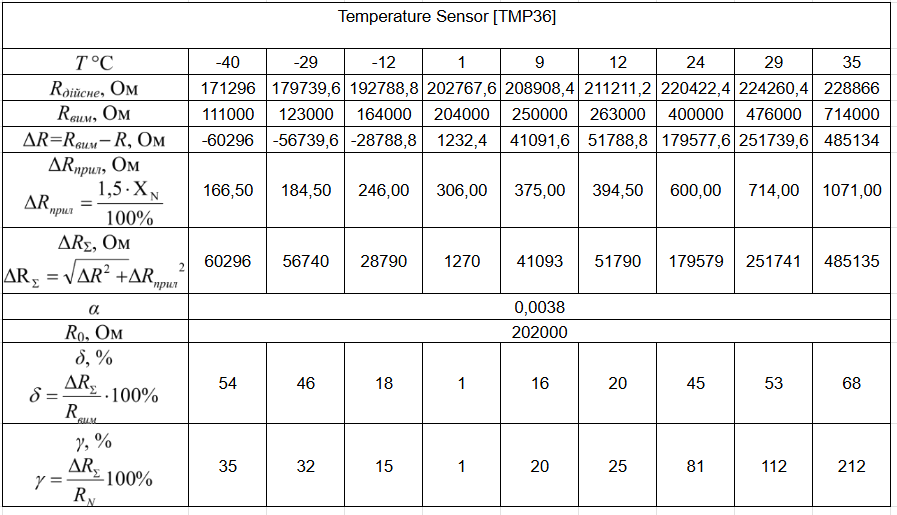
\includegraphics[width=1\textwidth]{imgs/LW3.1.png}
    \caption*{Рис. 3.1: Результати обчислень}
\end{figure} 

\begin{figure}[h]
    \centering
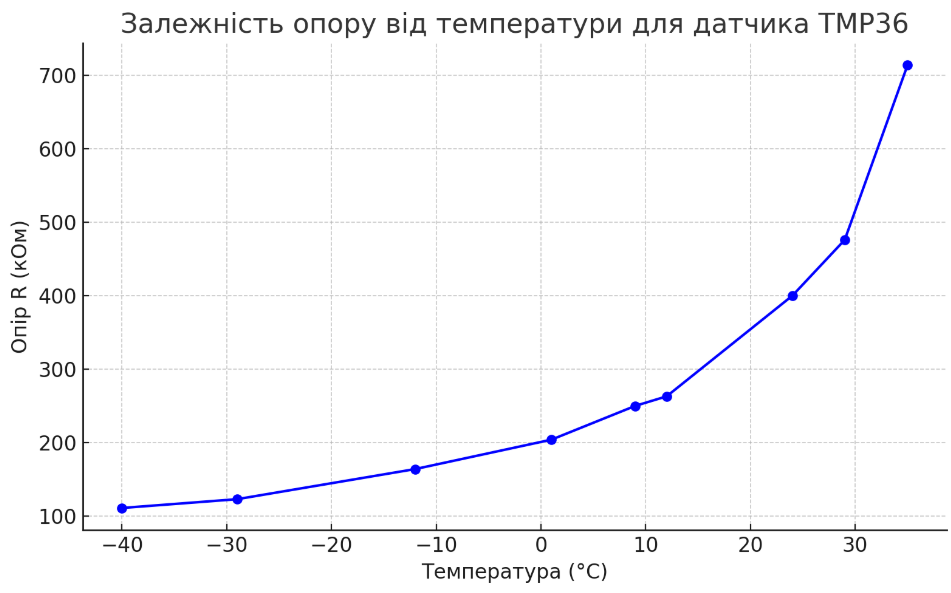
\includegraphics[width=0.8\textwidth]{imgs/LW3.2.png}
    \caption*{Рис. 3.2: Таблиця залежності опору від температури}
\end{figure} 

\newpage
\section*{Висновки}
В ході роботи було досліджено характеристики терморезистора, визначено його статичну характеристику та чутливість. Одержані результати відповідають теоретичним уявленням про роботу резистивних перетворювачів температури.

\section*{Контрольні питання з відповідями}
\begin{enumerate}
    \item \textbf{Що таке терморезистори і для чого вони використовуються?}\\
    Терморезистори — це резистивні перетворювачі, які змінюють свій опір залежно від температури. Вони використовуються для вимірювання та контролю температури у різних технічних і промислових процесах.
    
    \item \textbf{Які датчики температури Ви знаєте? У чому різниця між ними?}\\
    Датчики температури поділяються на терморезистори, термопари, ртутні та спиртові термометри, пірометри. Основна різниця між ними — принцип роботи: терморезистори змінюють опір, термопари генерують термо-ЕРС, а ртутні та спиртові термометри використовують розширення рідини.
    
    \item \textbf{Яка залежність опору металевого терморезистора від температури?}\\
    Опір металевого терморезистора збільшується лінійно зі зростанням температури згідно з формулою $R = R_0 (1 + \alpha t)$.
    
    \item \textbf{Що таке температурний коефіцієнт опору терморезисторів?}\\
    Це коефіцієнт, що характеризує відносну зміну опору терморезистора при зміні температури на 1°С.
    
    \item \textbf{Чому термістори застосовуються рідше порівняно з металевими терморезисторами?}\\
    Термістори мають нелінійну характеристику, що ускладнює калібрування та обчислення температури, тоді як металеві терморезистори мають лінійну залежність.
    
    % \item \textbf{Наведіть приклади практичного застосування терморезисторів.}\\
    % Терморезистори використовуються для контролю температури підшипників, двигунів, електронних пристроїв, систем охолодження та обігріву.
\end{enumerate}

\end{document}